\chapter{Testing and Evaluation}
\section{Introduction}

This section will detail my plans on how I will test my solutions, and how I will determine how they have measured up against the specifications defined for them.

TODO: emphasis on the framework, not the example usage of the framework. How to test the framework with these pieces as an example

There will be two main testing approaches throughout the project, individual Unit Testing on different components of the software, and more end-user oriented end-to-end testing where I will be actual using the functionality and deeming it functional. 
\section{Unit Testing with SuperTest, Jest and Nock}

My Unit Tests for both the micro-service and the client will use a number of key libraries, SuperTest, Jest and Nock. Whilst they will test the sample services I have created, the main aim will be to produce a suite of tools for general micro-service testing.
\subsection{SupertTest}
SuperTest is a Node.js library used for testing HTTP. By passing in the server export from the App.ts we can perform Unit Tests on the actual HTTP requests made through the server.

All aspects of the response can be tested including headers and status code, with the body of the response being the focal point of my testing. This will allow me to ensure that everything returned by the API is returned in both the format and shape that is expected, and the appropriate errors are thrown on respective requests.
\subsection{Jest}
Jest is a lightweight and very user-friendly JavaScript testing framework developed by Facebook. The tests themselves are split into separate processes and run in parallel, resulting in extremely fast and performant test suites.

Jest requires very little boilerplate configuration, and pretty much works out of the box making it very easy to get straight to writing Unit Tests on the code-base.

The framework also has the Istanbul code coverage tool built in. Istanbul tracks how much of our code is actually covered by our Unit Tests such as:
\begin{itemize}
    \item Functions: Are all the functions and methods tested
    \item Branching: Are all branches in the decision-making logic tested
    \item Statements: Are all variable assignments, return values etc tested
\end{itemize}

The reports generated by Istanbul detail what code isn't covered too, allowing the test suite to be expanded to cover these areas. The high the code coverage, the more of the code-base that is tested, which in turn should reduce the numbers of bugs introduced to the system.

It should be noted that Code Coverage and Test Coverage are different. Where Code Coverage tests how much of the code is tested in some way, Test Coverage measures those tests against actual Specifications and Requirements, testing the actual coverage of the expected functionality. As such where Code Coverage shines for Unit Tests, Test Coverage is a very good metric for Acceptance Testing.

For this project I will only be testing Code Coverage as the bulk of my physical tests will be Unit Tests.
\subsection{Nock}
Nock is a Node.js library used for mocking HTTP requests. Nock intercepts the HTTP requests sent by the server or application, and rather than actually forwarding the error to the destination it returns a static response body or error defined by the developer. 

It is particularly useful for interacting with external APIs as it mimics the request sent by the consuming service without actually interacting within the API. This allows the unit tests to be run without connecting to the internet or running any of the dependencies of the service being tested locally. 

Nock allows creation of highly configurable mocks and every component of the requests and responses can be tweaked. This includes everything from headers to status codes.

Once a request is intercepted the mock is consumed. This allows different instances of the exact same request to return different responses. This is particularly useful for testing things like rate limit handling, as the first few requests which are limited will fail with a 429 status code, but subsequent requests that are not limited will return successfully.

All of the unit tests for my API Client will make use of Nock so that it can be tested in isolation from the micro-service.
\subsection{Code Coverage Target}
Oftentimes it can be extremely challenging to hit one hundred percent code coverage. While I will aim to hit as close to complete coverage as possible, I will be aiming for a minimum of eighty five percent of overall code coverage for both the client and micro-service. There are likely to be certain parts of the code that aren't feasible to reach during unit-testing, particularly around handling of unexpected failures around the database connections.
\subsection{Unit Testing the Micro-service}
The testing of the micro-service will be broken down into two key sections, testing that the controllers work and respond as expected, and that the data-agents process and store the data correctly.
\subsubsection{Testing the Controllers}
In order to test the controllers and the REST API exposed through them I will make use of the SuperTest library. SuperTest allows programmatic HTTP requests to be made to the server within the unit tests, allowing testing of the same URL endpoints that the live API will expose.

Upon calling the HTTP requests I will use Jest assertions to verify that the fields returned within the response are correct. To do this I will have to create static response bodies for each of the requests that I wish to test and compare them against those actually returned by the request. If the fields match those expected, then the API is working as expected.

Each of the URL endpoints within the micro-service will have a small suite of unit tests written for them. Requests that should trigger successful responses will be validated as will as requests that should trigger expected errors, such as doing GET requests on resources that do not exist. The HTTP status codes will be tested, ensuring that they are being assigned correctly and any response or error bodies will also be checked to ensure that they contain all of the content that they should. Essentially any documented request and response for the API should be tested.
\subsubsection{Testing the Data Agents \& Models}
Testing the data-agents and models involves interacting with the actual database operations. We do not want our unit tests ever interacting with live data and so standard practise is to connect to a completely separate test-focused database. This is easy to do with Mongoose, and we can simple create a new database connection as part of the unit tests. Once the database connection is defined we can simple inject a number of test documents into the collections to act as our test data.

A small sample of test documents will be created upon the start up of the unit tests and saved into the test database. Different values for each of the model fields will be used across the suite of documents. This will allow tests to be written that verify that the correct subset of the collection is returned for the different filtering and sorting options on the data-agent methods.

Each of the operation involved in fetching existing documents will utilise the test documents created upon database startup. This will allow assertions to be run against the actual document definitions reducing boilerplate and keeping the unit tests lightweight. However, for the operations involving modifying or creating documents the tests will consist of two stages. The first will be defining the parameters used for the creation or modification or the resource, as well as creating a JSON representation of the resource after the operation has been defined. The method can then be called assertions can be tested to ensure that the operation did not fail. In order to test that the actual data saved is what is expected, a second request fetching the new data needs to be made. This can be done directly through the mongoose model using the primary key used in the create or modify operation, and the response can be tested against the previously defined JSON object. This two-stage process ensures that not only does the operation not fail, the actual information stored in database is exactly what is expected.
\subsection{Unit Testing the Handcrafted Client}
Testing the client will involve using Nock to intercept and mock the responses of all the outgoing requests that the client sends out. These will simulate both successful and failed requests and allow all expected cases to be tested against.
\subsubsection{Intercepting HTTP Requests to the micro-service with Nock}
There are a number of different behavioural aspects that need to be tested within the client. The successful responses need to be properly handled and parsed into objects that are expected, any errors thrown by the API need to be caught and handled without losing any crucial information and certain failed requests need to be retried automatically.

Testing handling of sucessful responses is easy with Nock. The endpoint simply need to passed into the Nock constructor before calling the \textit{.reply()} method with both the status code and response body that the mocked request should return. An example can be seen below.
\begin{verbatim}
    const request = Nock('http://localhost:3000/REST/1.0')
    .get('/shoppingItems') 
    .reply(200,
        {
            page: 1,
            totalPages: 1,
            shoppingItems: [{
                "name":"apple",
                "category":"Fruit",
                "numberOfStock":110,
                "inStock":true
            }]
        })
    const res = await client.getShoppingItems();
\end{verbatim}
The above code simply initialises a new variable \textit{request} and assigns it to the request made to the \textit{"/shoppingItems"} endpoints. The spoofed response is assigned the status code 200, imitating a successful operation, and an example of the correct response payload is also injected in. The \textit{getShoppingItems()} can then be called. As far as the methods calling the endpoints are concerned they will have interacted with what they believe to be the live API, but behind the scenes the request will have been intercepted and replaced with the Nock. The consuming code will then treat the faked response the same as a legitimate one and the outputs of the methods can be asserted against to check that they are working correctly.

Failed requests can be built and used in the exact same way. A status code and an error payload just need to be assigned to the Nock request to endpoint and it's good to go.
\begin{verbatim}
    const failedRequest = Nock('http://localhost:3000/REST/1.0')
    .get('/shoppingItems/mango')
    .reply(404, 
        {
            "errorIdentifier": "ShoppingItemNotFound",
            "message": "Shopping Item not found with params: 
                {
                    \"name\":\"mango\"
                }"
        })
    const res = await client.getShoppingItem('mango');
\end{verbatim}
The code above simply creates a Nock imitating a request made for a resource that does not exist. The method that consumes the request is expected to throw an instance of the \textit{ErrorWrapper} object using the data from the error payload and status code. The unit tests for the failed requests will test that the expected object is thrown and that it contains the fields and values that are expected. This is easily done through simple assertions on the object properties within the unit tests.

Once a request has been intercepted and assigned a matching Nock, the Nock is consumed. Any subsequent requests will need to have separate Nock objects assigned to them. This allows the automatic retry facilities of the client to be tested quite easily. The rate limit retry system works by making the first request, checking the status code returned in the case of an error and if supported, a number of retries of the same request will be made with incremental delays between them. Essentially a successful retry system will contain a number of failed requests, followed by a final successful request. With Nock we can define all of these requests and the system should handle them as if they were interacting with an actual rate-limited API. An example for testing a request made successfully after three retries is given below.
\begin{verbatim}
    const failThrice = Nock('http://localhost:3000/REST/1.0')
    .get('/shoppingItems')
    .times(3)
    .reply(429)
    const retriedSuccessRequest = Nock('http://localhost:3000/REST/1.0')
    .get('/shoppingItems') 
    .reply(200,
        {
            page: 1,
            totalPages: 1,
            shoppingItems: [{
                "name":"apple",
                "category":"Fruit",
                "numberOfStock":110,
                "inStock":true
            }]
        })
    const res = await client.getShoppingItems();
\end{verbatim}
There are two Nocks defined above. The first behaves the same as the previous spoofed errors with one exception, it has the additional \textit{.times()} function call attached. All this does it tell Nock that the request should exist three times. This means that when the axios-retry library makes retries the request after the initial failure, it will receive two subsequent rate-limited errors. 

The second Nock is a typical successful mocked response for the same endpoint. When the retry is triggered a third and final time this response will be returned. When the \textit{getShoppingItems()} method is called the output should contain the information provided by the final success. As with the previous tests this can be tested by simple asserting the fields provided in the response body outputted by the method.
\section{End-to-End Testing the Auto-generated Client}
\subsection{Migrating the Unit Tests from my Client}
In order to test the auto-generated client I will pull out the unit tests from my custom client, and copy them across into the generated client. The tests will require some very light modification but all of the Nock descriptions and assertions on the responses should be transferable. The only modifications should be changes to the names of methods called and any variance in the method signatures.

The clients package.json file will also need some additional libraries to be imported in order for the unit tests to run, however this will have no bearing on the actual functionality of the client. These will include the Jest framework and Nock library.
\section{Results of the Tests}
In this section I will analyse the Code Coverage reports generated for each of the services to get a general idea of how the test suites truly test the code.
\FloatBarrier
\subsection{The Micro-service}
Overall the coverage for the micro-service was very comprehensive and the target coverage of 85\% was exceeded. Figure 6.1 below shows the full breakdown of the report produced by Jest.
\begin{figure}[!htb]
\caption{Code Coverage Report for the Exemplar Micro-service}
\centering
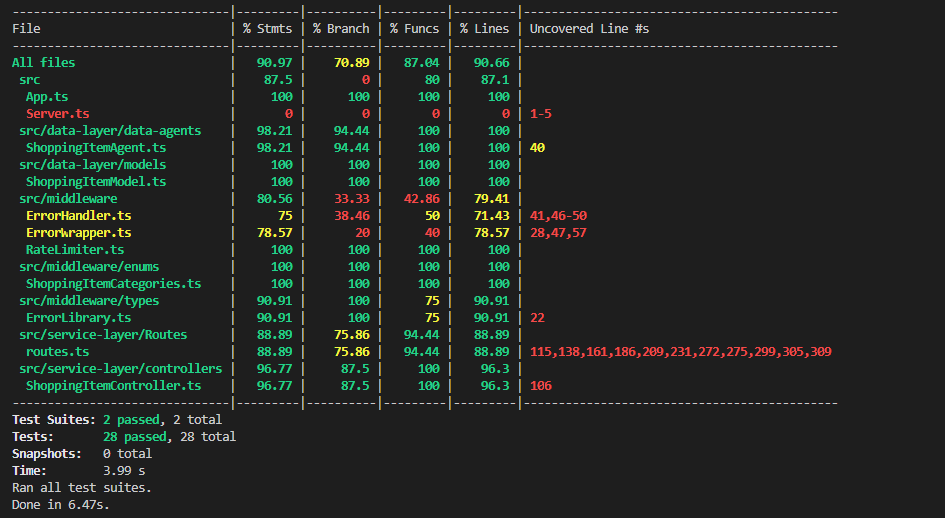
\includegraphics[scale=0.62]{FYP_Dissertation_template/Figures/microservice-code-coverage.PNG}
\end{figure}
\FloatBarrier
When writing the unit-tests for the micro-service the key areas of interest where the data-agents, models and controllers. This is where the vast majority of the business logic is stored including the database interactions, data processing and HTTP request and response handling. The coverage on these files is close to 100\% coverage, with only a couple of lines of code not explicitly covered within the ShoppingItemController and ShoppingItemAgent. The report tells us exactly what line is not covered in each file and upon further inspections we can see that it is code relating to the handling of uncaught exceptions, something very hard and not really worth testing for. The report shows us that all of the code that we wanted tested within the files has been covered by the test suite and so we can have a certain degree of confidence within the code. Additionally the coverage on the RateLimiter file is 100\% which again gives confidence in the RateLimiting aspect of the service. The pagination is handled across the models and data-agents and the code handling this functionality is also fully covered by the unit-tests.

In general the vast majority of logic within the application has been tested, the only real gaps in the coverage is relating to exceptions happening out of the blue around the database, and subsequent handling of the error has a HTTP response with a 500 status code.
\subsection{The Handcrafted Client}
Figure 6.2 shows the report for the Code Coverage of my custom API client. Again, the break-point of 85\% coverage has been exceeded with a total coverage of 91\% for the client.
\begin{figure}[!htb]
\caption{Code Coverage Report for the Handcrafted Client}
\centering
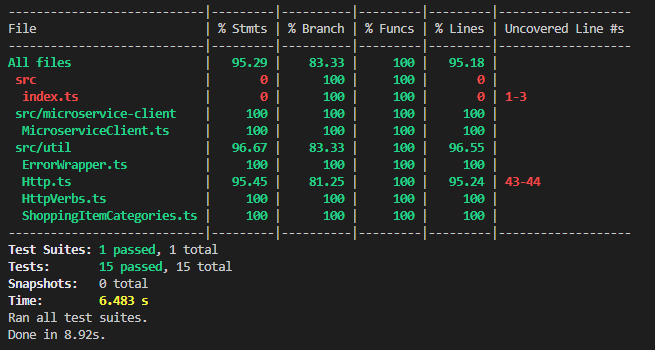
\includegraphics[scale=0.70]{FYP_Dissertation_template/Figures/handcrafted-client-code-coverage.PNG}
\end{figure}
Taking a further look at the report we can see the actual MicroserviceClient file has 100\% code coverage. This file exposes the actual URL endpoints and parameters to the user of the client and full coverage shows that all interactions with the API client are tested, including expected error cases. 

The Http file handles the actual logic of making the requests to the API. Whilst it only has a total code coverage of 88\% if we take a look at the lines not covered we can see that once again they are related to the handling on completely unexpected errors. The actual business logic of the HTTP request and response handling are fully covered. This includes all of the functionality around automatically retrying certain failed requests and the the correct handling of HTTP errors thrown by the API.

The rest of the files are relatively unimportant and only really act as Enumerated types or Type definitions. Despite this coverage of these files is 100\%.

\subsection{The Auto-generated Client with the modifications}
The report for code coverage of the API client generated from the OpenAPIGenerator templates I modified are shown in Figure 6.3. The unit-tests were pulled out of my handcrafted client and so with some very minor method signature changes, the test-suite itself is identical across the two clients.

\begin{figure}[!htb]
\caption{Code Coverage Report for the Generated Client with my Modifications}
\centering
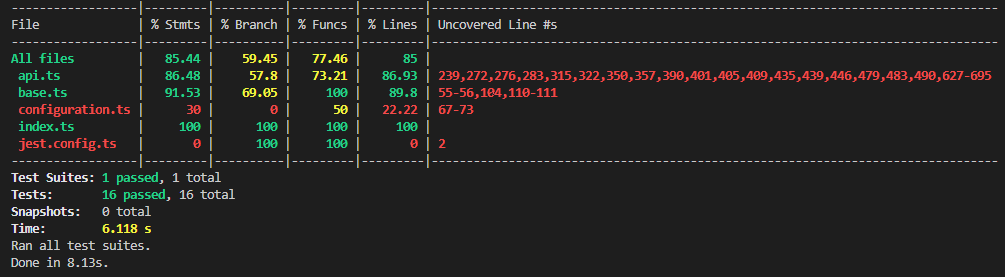
\includegraphics[scale=0.55]{FYP_Dissertation_template/Figures/modified-client-code-coverage.PNG}
\end{figure}

Despite sharing the same test-suite, the coverage of the two clients are fairly different. The file structure and code architecture of the clients are vastly different, and the OpenAPISpecification client has a number of extra feature sets baked into the client such as OAuth and Token authorisation handling. As my API does not make use of these features there are no tests covering them, and as such coverage is lower. The important thing is that the tests pass, which all of them do. This shows that the additonal functionally around the automatic request retries and error handling works within the generated client.

The test-suite for the generated client includes one extra unit-test around the OpenAPIGenerators handling of the createShoppingItem() method when no body payload is passed in. Whilst the additional test is unnecessary, I added it just to make sure my modifications didn't break the existing handling of the error format it uses.
\section{Evaluation against Project Objectives}
In this section I will look back at the objectives for the project and determine whether they have been met for each piece of software.
\subsection{The Exemplar Micro-service}
In order to assess how well the framework meets the project objectives, we will now evaluate them against the exemplar micro-service. This is a simple service that could be used by any shopping application and is designed to showcase the combinations of libraries that would be used in any real micro-service.
\subsubsection{The Objectives for the Micro-service}
\begin{enumerate}
    \item \textit{Generate an OpenAPI Specification file}
    \item \textit{Use well-formed URLs}
    \item \textit{Provide endpoints for each of the major HTTP verbs}
    \item \textit{Assign the correct HTTP status codes to both Success and Error Responses}
    \item \textit{Validate both request and response payloads}
    \item \textit{Provide useful documentation for the API}
    \item \textit{Utilise Rate Limiting}
    \item \textit{Make use of Pagination on large responses}
    \item \textit{Provide access to a database to support CRUD usage of different HTTP Verbs}
\end{enumerate}
\subsubsection{Generate an OpenAPI Specification file}
The TSOA library provides the facilities for taking the API definitions defined into the controller files and generates an OpenAPI Specification file from them. It does this through the command:
\begin{verbatim}
    yarn run tsoa spec
\end{verbatim}
The output from this command is either a YAML or JSON OpenAPI Specification.
\subsubsection{Use well-formed URLs}
When designing the ShoppingItem API for my micro-service, the API design best practices stated in Chapter 2 were used as a basis.

Those best practises are as follows:
\begin{enumerate}
    \item Resources should be named with nouns
    \item Resource names should be pluralised
    \item Individual resources should be fetched through use of identifiers
\end{enumerate}
The base URL for the REST API is the following:
\begin{verbatim}
    /REST/1.0/shoppingItems
\end{verbatim}
By looking at the URL we can see that the ShoppingItem resource is named after a noun, and the noun is in it's plural form.

The API endpoint for fetching an individual Shopping item is:
\begin{verbatim}
    /REST/1.0/shoppingItems/{name}
\end{verbatim}
The endpoint is an extension of the base URL, where {name} is the unique name of the targeted individual resource. This name acts as the unique identifier for the resource which in turn checks of the third best practice.
\subsubsection{Provide endpoints for each of the major HTTP verbs}
There are four major HTTP verbs that this objective is referencing: GET, POST, PUT and DELETE. Each of these verbs have associated endpoints within the ShoppingItems API.
\begin{enumerate}
    \item GET
    \begin{verbatim}
        /REST/1.O/shoppingItems
        /REST/1.0/shoppingItems/{name}
    \end{verbatim}
    \item POST
    \begin{verbatim}
        /REST/1.0/shoppingItems
    \end{verbatim}
    \item PUT
    \begin{verbatim}
        /REST/1.0/shoppingItems/{name}/category
        /REST/1.0/shoppingItems/{name}/increaseStock
        /REST/1.0/shoppingItems/{name}/decreaseStock
    \end{verbatim}
    \item DELETE
    \begin{verbatim}
        /REST/1.0/shoppingItems/{name}
    \end{verbatim}
\end{enumerate}
\subsubsection{Assign the correct HTTP status codes to both Success and Error Responses}
Correctly assigning HTTP status codes are crucial if consumers are going to successfully use the REST API. The micro-service API follows the standardised assignment of status codes explored in Chapter 2.

Success responses for any request that returns a resource  are assigned a 200 status code alongside the response body. For the creation of a new resource the status code 201 is assigned and a 204 status code is used when a resource is deleted.

When a resource is not found a status code of 404 is used, and in the case of a bad request 400 is used. Any unexpected error on the server side is assigned a 500 status code. A request that breaks the rate limits of the API is assigned a 429 status code.
\subsubsection{Validate both request and response payloads}
The TSOA library is used for creating all of the routing and API generation for the micro-service. Out of the box TSOA handles all of the validation for the API endpoints, using TypeScript types to validate both incoming and outgoing payloads and blocking any that do match the expected format.

When an endpoint is defined that takes in a request body, such as the endpoint associated with the creation of a new ShoppingItem, the body is cast as a TypeScript type. When a request hits the API endpoint TSOA takes the body from the HTTP message and compares it to the assigned type. If there are missing required fields, has unexpected fields or the body is of an unexpected format then it will throw a ValidationError with a 400 status code to the consumer.

Similarly the response body is defined by a TypeScript type and assigned to the return type of the controller method associated with the endpoint. As TypeScript is a strongly-typed language this tightly weaves the response into the lower level code handling the business logic of the request. If the method that the controller calls returns a different type then TypeScript itself will thrown an error on compile time.
\subsubsection{Provide useful documentation for the API}
The micro-service has the ability to generate an OpenAPI Specification representing a full definition of it's API. The swagger-ui-express library takes this document and parses it into a HTML page fully detailing the endpoints using the information provided in the specification. An API endpoint that serves this page can be assigned to the server, allowing the creation of a full documentation endpoint that any user can hit to get the details of the API.

Whilst this library generates the actual page, it works in tandem with TSOA. When TSOA generates the OpenAPI specification it scours the types and methods used for both additional decorators and JSDoc notation. These optional additions to the files allows developers to add a large volume of extra information and descriptions to various fields, methods and payloads. This extra data is then injected into specification file. By documenting the code itself, developers can automatically generate fully descriptive API documentation.
\begin{figure}[!htb]
\caption{Documentation snippet from the micro-service documentation URL}
\centering
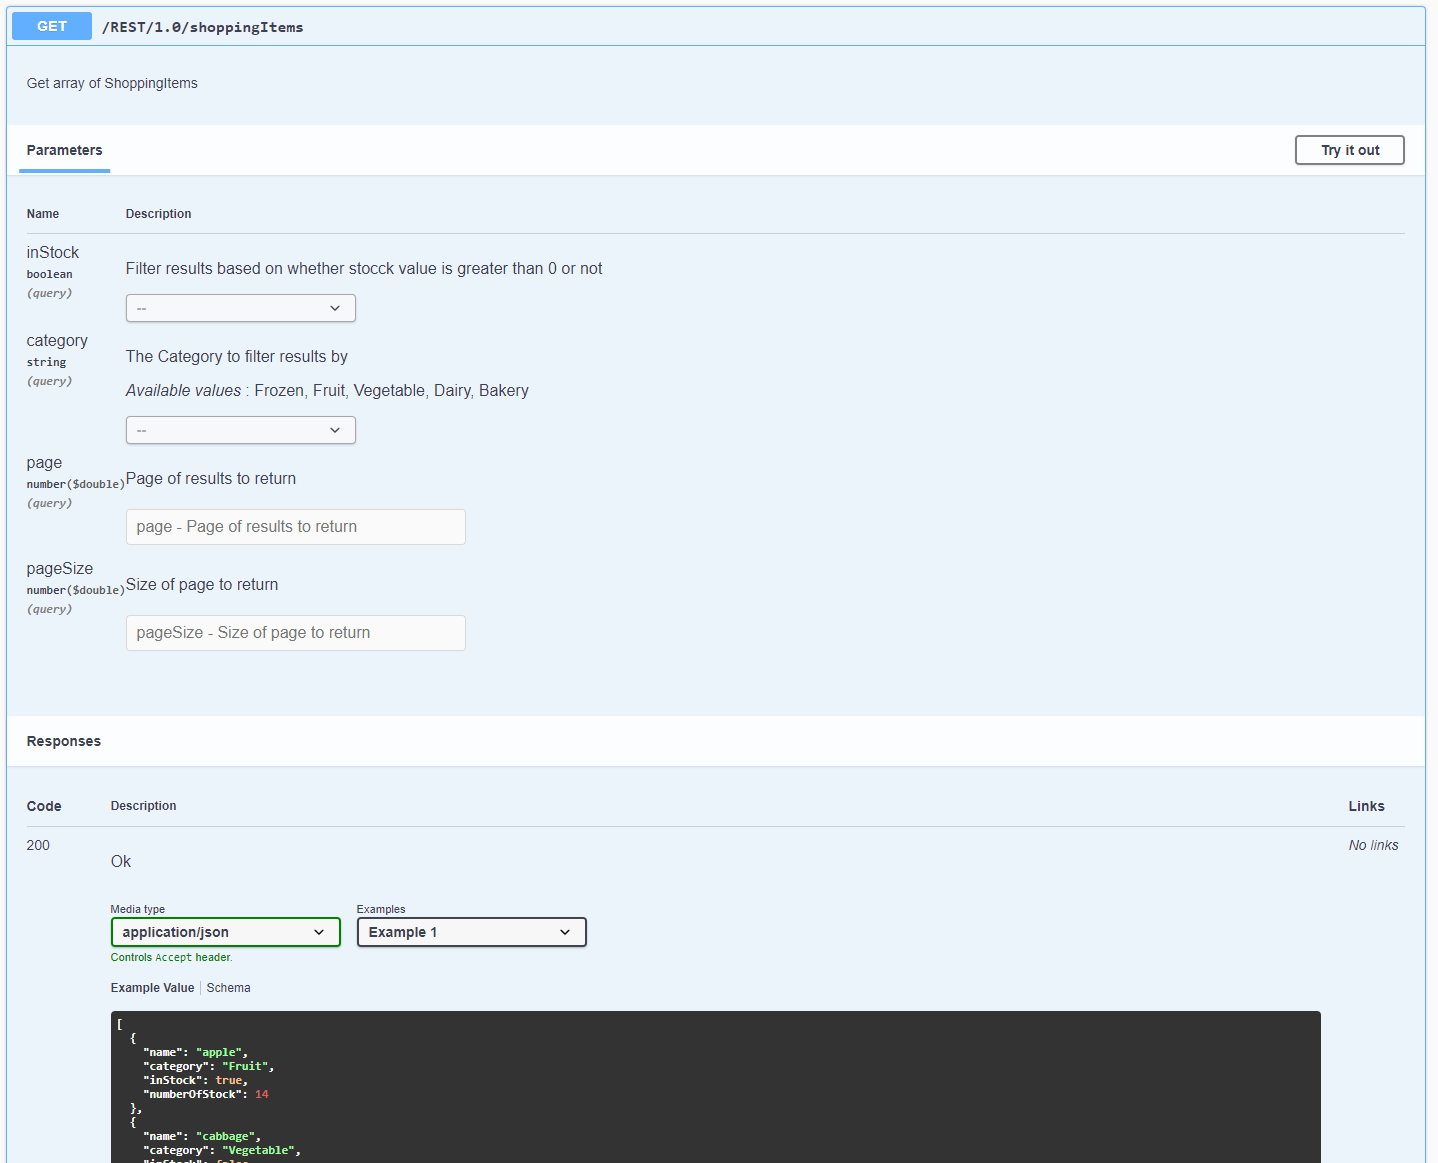
\includegraphics[scale=0.41]{FYP_Dissertation_template/Figures/doc-example.PNG}
\end{figure}
\FloatBarrier
Figure 6.4 above shows part of this HTML page. Information relating to each of the query parameters, an overall endpoint description and example response payload are provided.

Outside of acting as documentation, the swagger-ui-express library also allows requests to be made directly through the web-page, saving time writing complex and tedious CURL commands when testing the API.
\subsubsection{Utilise Rate Limiting}
The express-rate-limit library is used to add rate-limiting functionality to the micro-service. Whilst it is a relatively simple integrations, applying a global rate limit to the service rather than a per user limit, it works fine as a proof of concept. Outside of intercepting requests that would break the limit and throwing a 429 error, it also inject a number of rate limit meta-data headers into the responses of the API.
\begin{figure}[!htb]
    \caption{Example of Rate Limit response headers provided by the API}
\centering
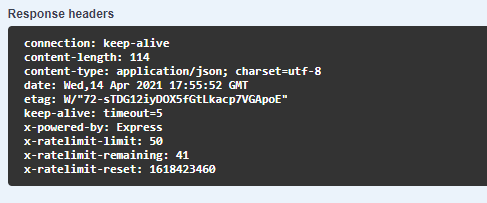
\includegraphics[scale=0.6]{FYP_Dissertation_template/Figures/rate-limit.PNG}
\end{figure}
\FloatBarrier
The above figure shows the response headers include information about the rate limit itself, number of remaining requests before the limit is exceeded and a timestamp for when the current limit expires. This information can be used by the API consumer in order to request any failed requests, or plan how to make a series of requests to the API.
\subsubsection{Make use of Pagination on large responses}
\subsubsection{Provide access to a database to support CRUD usage of different HTTP Verbs}

\subsection{The Handcrafted Client}
Text goes here...
\subsubsection{The Objectives for the Handcrafted Client}
\begin{enumerate}
    \item \textit{Support all endpoints across the API}
    \item \textit{Provide details of the responses types returned by endpoints}
    \item \textit{Provide details of all input parameters for the endpoints}
    \item \textit{Ensure all important error information is correctly is passed on}
    \item \textit{Automatically retry requests that fail with certain HTTP status codes}
\end{enumerate}
\subsubsection{Support all endpoints across the API}
\subsubsection{Provide details of the responses types returned by endpoints}
\subsubsection{Provide details of all input parameters for the endpoints}
\subsubsection{Ensure all important error information is correctly is passed on}
\subsubsection{Automatically retry requests that fail with certain HTTP status codes}
\subsection{The Auto-generated Client}
Text goes here...
\subsubsection{The Objectives for the Auto-generated Client}
\begin{enumerate}
    \item \textit{Support all endpoints across the API}
    \item \textit{Provide details of the responses types returned by endpoints}
    \item \textit{Provide details of all input parameters for the endpoints}
    \item \textit{Ensure all important error information is correctly is passed on}
    \item \textit{Automatically retry requests that fail with certain HTTP status codes}
\end{enumerate}
\subsubsection{Support all endpoints across the API}
\subsubsection{Provide details of the responses types returned by endpoints}
\subsubsection{Provide details of all input parameters for the endpoints}
\subsubsection{Ensure all important error information is correctly is passed on}
\subsubsection{Automatically retry requests that fail with certain HTTP status codes}